\documentclass[twocolumn,english]{IEEEtran}
\usepackage[T1]{fontenc}
\usepackage{babel}
\usepackage{amsthm}
\usepackage{amsmath}
\usepackage{graphicx}
\usepackage[unicode=true,
bookmarks=true,bookmarksnumbered=true,bookmarksopen=true,bookmarksopenlevel=1,
breaklinks=false,pdfborder={0 0 0},backref=false,colorlinks=false]
{hyperref}
\usepackage{bm}
\usepackage{amsmath}
\usepackage{amssymb}
\usepackage{natbib}
\usepackage{array}
\usepackage{calc}
\newcolumntype{W}{>{\centering\arraybackslash}m{25mm}}
\newcolumntype{L}{>{\centering\arraybackslash}m{15mm}}
\makeatletter
\setcounter{topnumber}{2}
\setcounter{bottomnumber}{2}
\setcounter{totalnumber}{4}
\renewcommand{\topfraction}{0.85}
\renewcommand{\bottomfraction}{0.85}
\renewcommand{\textfraction}{0.15}
\renewcommand{\floatpagefraction}{0.7}
\usepackage{float}
\usepackage{booktabs}

\hypersetup{
pdftitle=  {Lab 4: Diode Circuits},
pdfauthor= {Alex Landry, Nolan Guettler, Zack Garza}%TODO: Fill in names
pdfpagelayout=OneColumn, pdfnewwindow=true, pdfstartview=XYZ, plainpages=false}

\begin{document}

\title{Lab 4: Diode Circuits}
\author{Alex Landry, Nolan Guettler, Zack Garza} %TODO: Fill in names
\IEEEspecialpapernotice{Engineering 17L \\ Effective Date of Report: \today}

\markboth{Lab 4: Diode Circuits}{Zack Garza}
\maketitle

\begin{abstract}
\IEEEPARstart{D}{iodes} are crucial elements in modern circuitry. They work like one-way gates for current, and have a wide array of electrical applications. This report investigates several circuits which utilize both diodes and zener diodes,  which allow one-way current travel until a certain maximum is reached. Several circuits that utilize these diodes are examined, including clipping circuits, clamping circuits, voltage regulator circuits, AC to DC conversion circuits, and circuits that implement digital logic.
\end{abstract}

\tableofcontents

\section{Equipment List}
\begin{enumerate}
  \item Breadboard
  \item \underline {Measuring Equipment:}
    \begin{enumerate}
      \item Digital Oscilloscope
      \item Digital Multi-Meter \hfill[x2]
    \end{enumerate}
  \item \underline {Power Sources:}
    \begin{enumerate}
    \item DC Power Supply
    \item Function Generator
    \end{enumerate}
  \item \underline{Resistors:}
    \begin{enumerate}
    \item 1.0 k$\Omega$ (1/4 W) \hfill[x1]
    \item 10.0 k$\Omega$ (1/2 W) \hfill[x1]
    \item Variable Resistor Box
    \end{enumerate}
  \item \underline{Diodes:}
    \begin{enumerate}
     \item 1N4002 Diode \hfill[x2]
     \item 1N4737 Zener Diode \hfill[x1]
    \end{enumerate}
  \item \underline{Capacitors:}
    \begin{enumerate}
     \item 0.1 $\mu$F \hfill[x1]
     \item 1.0 $\mu$F (Electrolytic) \hfill[x1]
    \end{enumerate}
\end{enumerate}

\section{Methodology}

\subsection{Diodes as Clippers}
  \begin{enumerate}
    \item The circuit was built on the protoboard with $R_1=10$ k$\Omega$. %TODO: Need ref to diagram
    \item The oscilloscope was set to DC coupling mode, and Channels 1 and 2 were displayed simultaneously.
    \item A \textbf{1 kHz triangle wave} was used as the input signal. $V_{s1}$ and $V_{\text{Out 1}}$ were monitored on Channels 1 and 2 respectively.
    \item The following parameters of the input signal were varied, and the effects recorded:
      \begin{enumerate}
       \item DC Offset
       \item Frequency
       \item Peak-to-Peak Voltage
      \end{enumerate}
    \item Screen captures were generated that indicated the clipping behavior of the circuit.
    \item The second diode was wired parallel to the first to observe the resulting clipping effects. %TODO: Explain with diagram, labels?
    \item The following parameters of the input signal were varied, and the effects recorded:
      \begin{enumerate}
       \item DC Offset
       \item Amplitude
       \item Waveform Type
      \end{enumerate}
  \end{enumerate}

\subsection{Diode Clamping}
  \begin{enumerate}
   \item The circuit was built on the protoboard with $R_2 = 10$ k$\Omega$. %TODO: Ref to diagram
   \item A \textbf{1kHz sine wave} input signal was used, with the \textbf{DC Offset} set to \textbf{zero}.
   \item The oscilloscope was set to DC coupling mode. %TODO: Explain why DC coupling in results
   \item The oscilloscope was then wired to monitor $V_{s2}$ and $V_{\text{Out 2}}$.
   \item The input and output signals were measured on Channels 1 and 2 respectively. %TODO: Ref to diagram
   \item The DC Offset of the input signal was varied, and the effects on the output signal were measured and recorded.
  \end{enumerate}

\subsection{Voltage Regulator}
  \begin{enumerate}
   \item The circuit was built on the protoboard. %TODO: Ref to diagram, add exact values?
   \item A 20 V DC power generator was used as the source voltage.
   \item The oscilloscope was wired to measure the load variables $V_L$ and $i_L$.
   \item The resistance $R_L$ was varied, and data points were collected for both $V_L$ and $i_L$.
   \item A plot was generated of the data points as the experiment was conducted in order to determine where more data points were needed.
  \end{enumerate}

\subsection{AC $\rightarrow$ DC Converter} %Rightarrow causes error, but compiles. Only affects autogenerated table of contents in PDF.
  \begin{enumerate}
    \item The circuit was built on the protoboard. %TODO: Ref to diagram.
    \item The function generator was set to produce a \textbf{1 kHz sine wave}.
    \item The capacitor was tested for its polarization and connected appropriately.
    \item The oscilloscope was wired to measure $V_s$ and $V_{\text{Out}}$ on Channels 1 and 2 respectively.
    \item The oscilloscope was set to DC coupling on both channels.
    \item The oscilloscope was zeroed before capturing data. %TODO: Recalibrate? Or adjust levels?
    \item The resistance $R_L$ was varied, and the results were recorded.
    \item The voltages were measured with DVMs and recorded. %TODO: Which voltages?
  \end{enumerate}

\subsection{Diode Logic Circuits}
  \begin{enumerate}
   \item The circuit for the \textbf{AND} gate was built on the protoboard.
   \item A \textbf{5 V DC} power source was wired into the protoboard.
   \item The oscilloscope was wired to measure $V_{\text{Out}}$.
   \item Different combinations of voltages were applied to the inputs, and the outputs were recorded.
   \item The procedure was repeated for an \textbf{OR} gate.
  \end{enumerate}

\noindent\hrulefill


\section{Data and Analysis}

\subsection{\textbf{Clipping Circuit}}

\begin{figure}[h]
  \begin{centering}
  \begin{center}
  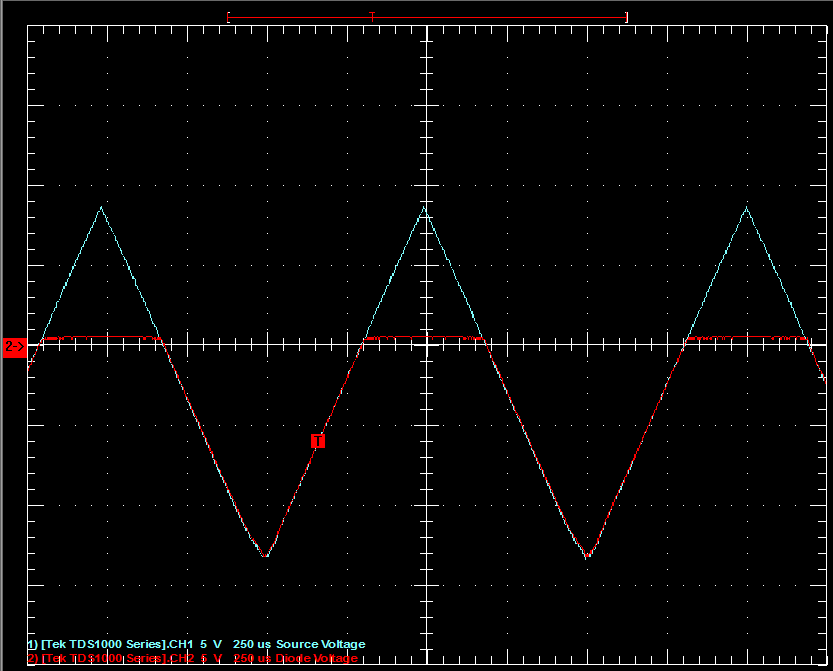
\includegraphics[width=\linewidth]{./Circuit_1.png}
  \caption{Source and diode voltage overlayed to show clipping behavior. The flat portion waveform just above the x-axis represents the clipped output voltage, while the triangle wave was used as the circuit's source signal.}
  \label{fig:circuit_1_results}
  \end{center}
  \par\end{centering}
\end{figure}

As the parameters outlined in the Methodology section were varied, the following observations were made, resulting in the waveforms shown in Figure~\ref{fig:circuit_1_results}.
\begin{enumerate}
  \item
    \textit{DC Offset}

    Changing the DC Offset of the signal generator changes the magnitude of the voltage supplied, but does not have a discernible effect on the output voltage. The diode effectively cut off the signal at approximately zero volts, regardless of what voltage was supplied by the source. \\

  \item
    \textit{Frequency}

    Changing the frequency of the source signal changes the edge behavior of the output voltage slightly.
    At low frequencies, the waveform of the output signal will mirror the input signal, with all voltages above zero rounded down to zero, which effectively flattens out the peaks.
    At higher frequencies, the source and output voltages begin to slip out of phase, and the waveform becomes sinusoidal with a peak at zero volts. \\

  \item
    \textit{Signal Amplitude}

    Increasing the amplitude of the source signal increases the steepness of the waveform of the output voltage, but does not have a large effect on the clipping behavior.
\end{enumerate}

It was found that the circuit deviated slightly from an ideal clipping circuit. While the theoretical maximum output voltage should be clipped to zero volts, the actual maximum output voltage was measured to be \textbf{552 mV}, which is shown in Figure~\ref{fig:cutoff_voltage}.
\begin{figure}[h]
  \begin{centering}
  \begin{center}
  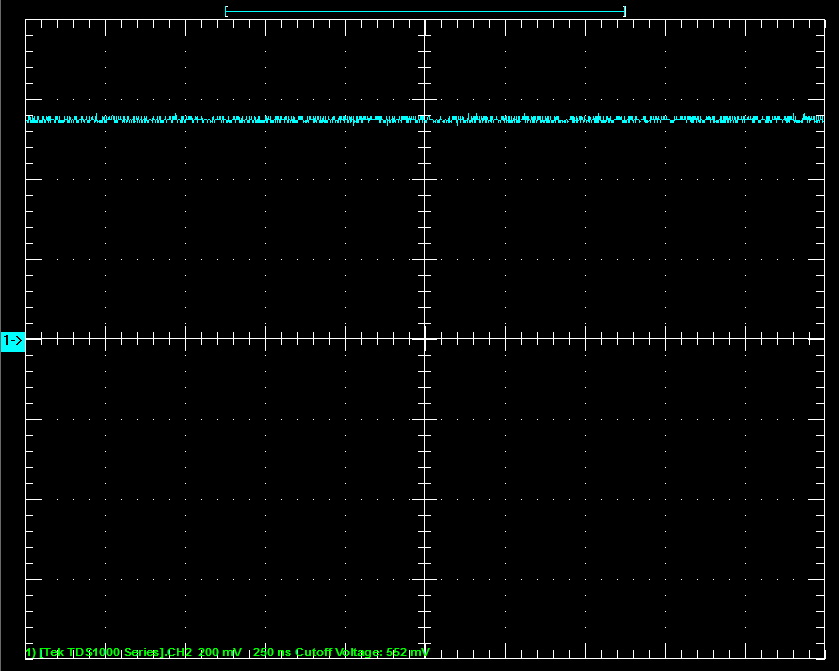
\includegraphics[width=\linewidth]{./Cutoff_Voltage.png}
  \caption{This is a zoomed in portion of the maximum clipped voltage, centered about zero. The deviation from zero volts was measured to be positive 552 mV, showing that the actual circuit behavior differs slightly from its theoretical ideal cutoff voltage.}
  \label{fig:cutoff_voltage}
  \end{center}
  \par\end{centering}
\end{figure}

\noindent\hrulefill
%%%%%%%%%%%%%%%%%%%%%%%%%%%%%%%%%%%%%%%%%%%%%%%%%%%%%%%%%%%%%%%%%%%%%%%%%%%%%%%%%%%%%%%%%
\subsection{\textbf{Clamping Circuit}}
The signal generated at the output terminals of the clamping circuit is nearly identical in form to the input signal, but shifted vertically until the peak signal voltage is above zero volts. The signal produced also tends to be less noisy, and easier to measure. As the parameters of the source and the oscilloscope were varied, the following observations were made:

\begin{enumerate}
  \item
    \textit{DC Offset}
    Increasing the DC offset increases the peak voltage of the source signal, effectively shifting it vertically upwards. However, changes in DC offset have virtually no effect on the output signal.
  \item
    \textit{Input Waveforms}
    The circuit preserved the shape and structure of the input signal almost perfectly. This behavior was characteristic of the circuit, regardless of whether a sine, square, or triangle wave was used.
  \item
    \textit{AC Coupling}
    Activating the ``AC Coupling'' option on the oscilloscope shifted both curves upwards significantly. However, it did not displace the input and output by equal values -- that is, both were shifted upwards by a different voltage. With this setting, it is not possible to compare the two signals effectively, and the clamping effect can not be seen.
\end{enumerate}

\begin{figure}[H]
  \begin{centering}
  \begin{center}
  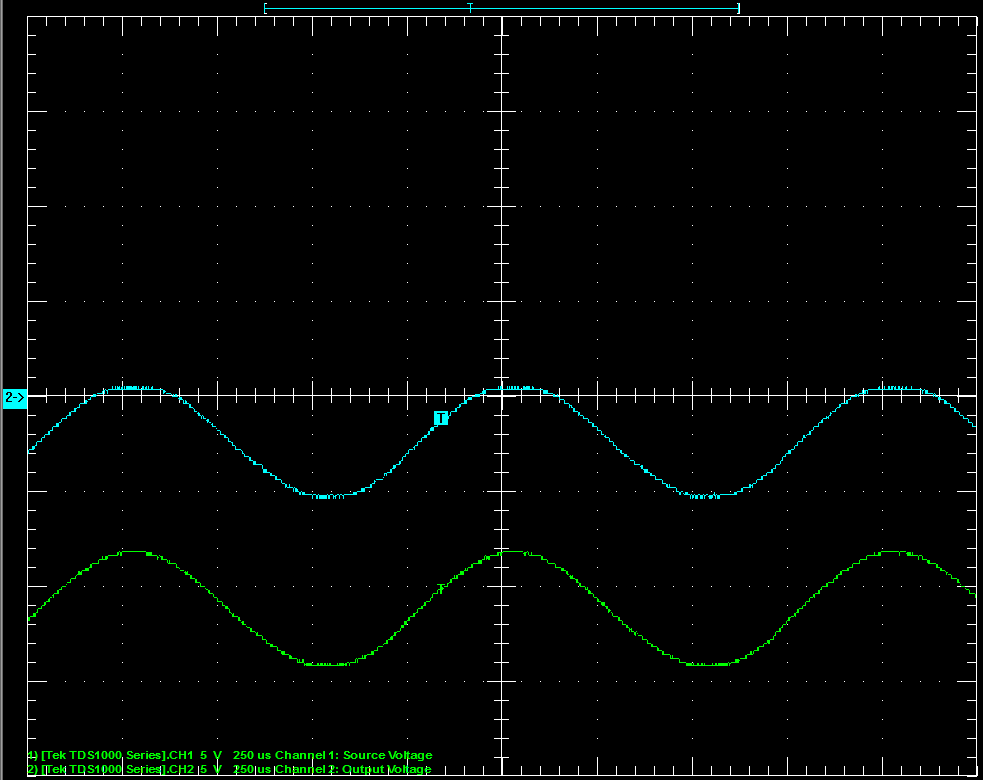
\includegraphics[width=\linewidth]{./clamping_results.png}
  \label{fig:clamping_results}
  \caption{Clamping Circuit}
  \end{center}
  \par\end{centering}
\end{figure}

\noindent\hrulefill
%%%%%%%%%%%%%%%%%%%%%%%%%%%%%%%%%%%%%%%%%%%%%%%%%%%%%%%%%%%%%%%%%%%%%%%%%%%%%%%%%%%%%%%%%
\subsection{\textbf{Voltage Regulator}}
From the $I-V$ curve shown in Figure~\ref{fig:voltage_reg}, the circuit was found to maintain a relatively constant voltage level across the output terminal over a range of currents. For load resistance values between 1.7 k$\Omega$ and 100 k$\Omega$, the voltage remained between 7 and 7.2 V. The breakdown voltage of the Zener diode, given by the data sheet, was 7.5 V, and thus in the range of loads tested, the output voltage agreed with the breakdown voltage to within 4\%.

The shape of the $I-V$ curve shows approximately where the diode's breakdown voltage occurs, which is represented by the vertical portion of the graph. This represents the current range over which the voltage delivered to the load is relatively constant. This an effective mechanism to limit the damaging effects of a poor or fluctuating power supply, as relatively large changes in current do not produce large voltage spikes or drops.

The $I-V$ curve bends as the resistance of the load is lowered, as more current is diverted through the load and the current through the zener diode drops below its minimum level. Below this level, the diode is no longer in a state of breakdown, and begins to function much like a normal diode.

\begin{figure}[H]
  \begin{centering}
  \begin{center}
  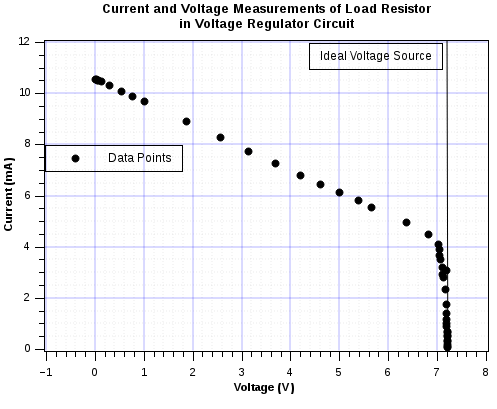
\includegraphics[width=\linewidth]{./voltage_reg.png}
  \caption{Plots of the load resistor's current and voltage, and its deviation from the behavior of an ideal voltage source.}
  \label{fig:voltage_reg}
  \end{center}
  \par\end{centering}
\end{figure}

\noindent\hrulefill
%%%%%%%%%%%%%%%%%%%%%%%%%%%%%%%%%%%%%%%%%%%%%%%%%%%%%%%%%%%%%%%%%%%%%%%%%%%%%%%%%%%%%%%%%
\subsection{\textbf{AC $\rightarrow$ DC Converter}}
This next circuit uses diodes and capacitors to level out an AC sine wave to approximate a DC source. First the diode connected to the positive terminal of the power supply makes the current only move in one direction, creating times of source current and times of no source current. During the time of source current the 1$\mu$F capacitor stores voltage. Then during the time of no source current, the capacitor discharges, creating a more level voltage source. The final component to this circuit is the zener diode.


\begin{figure}[h!]
  \begin{centering}
  \begin{center}
  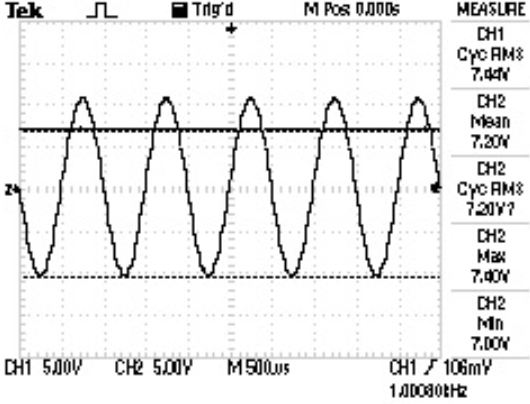
\includegraphics[width=\linewidth]{./dcp.png}
  \label{fig:dcp}
  \caption{AC to DC voltage conversion. The wave shown is the input signal, while the horizontal line is the output voltage that approximates a DC source.}
  \end{center}
  \par\end{centering}
  \end{figure}
The zener diode is like a pressure valve: if the voltage gets too high, the diode breaks down. This keeps the voltage across the load constant approximately around its breakdown voltage.

\begin{figure}[H]
  \begin{centering}
  \begin{center}
  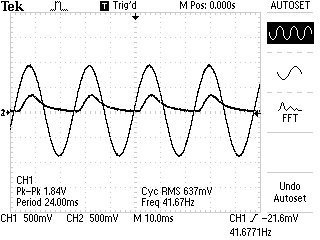
\includegraphics[width=\linewidth]{./DC1.png}
  \caption{Display of input and output signals. The output voltage is not strictly constant, as it exhibits an exponential voltage decay due to the capacitor.}
  \label{fig:DC1}
  \end{center}
  \par\end{centering}
\end{figure}

When the load resistance is lowered, the voltage across the Load decreases. The voltage across the zener diode connected in parallel with the load also decreases. If this voltage drops below the breakdown voltage, the voltage across the load will not be the breakdown voltage.

\begin{figure}[H]
  \begin{centering}
  \begin{center}
  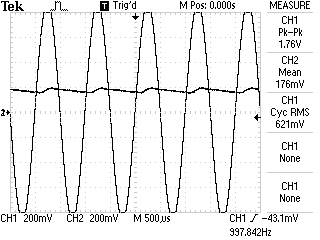
\includegraphics[width=\linewidth]{./DC2.png}
  \caption{As the frequency increases, the voltage drop between cycles decreases.}
  \label{fig:DC2}
  \end{center}
  \par\end{centering}
\end{figure}

When we increase the frequency of the source to 1 kHz, the output voltage levels out to the breakdown voltage of the zener diode. The voltage across the load using an ordinary DC volt meter gives us 7.12 V, while the oscilloscope measures the mean voltage across the load as 7.20 V. The supplied data sheet gives a breakdown voltage of around 7.5 volts.

\begin{figure}[H]
  \begin{centering}
  \begin{center}
  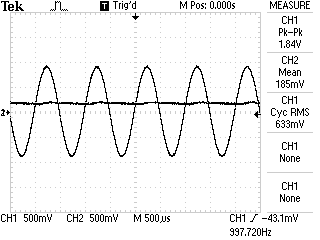
\includegraphics[width=\linewidth]{./DC3_5k.png}
  \caption{Zooming out at a high frequency shows that the output closely approximates a constant DC voltage.}
  \label{fig:DC3}
  \end{center}
  \par\end{centering}
\end{figure}

\begin{figure}[H]
  \begin{centering}
  \begin{center}
  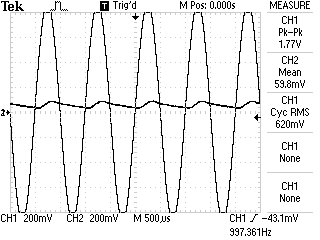
\includegraphics[width=\linewidth]{./DC4_1k.png}
  \caption{Changing the load resistance directly affects the voltage delivered to it. Decreasing the resistance by a factor of 5 lowered the output voltage by a factor of 3.}
  \label{fig:DC4}
  \end{center}
  \par\end{centering}
\end{figure}

The value the DC voltmeter gives us is \textbf{5\%} different then the data sheet and \textbf{1\%} different then the oscilloscope mean value. This may just be due to the internal resistance of the meter. Figures~\ref{fig:dcp} through~\ref{fig:DC4} show various aspects of the input and output signals of this circuit.

\noindent\hrulefill
%%%%%%%%%%%%%%%%%%%%%%%%%%%%%%%%%%%%%%%%%%%%%%%%%%%%%%%%%%%%%%%%%%%%%%%%%%%%%%%%%%%%%%%%%
\subsection{\textbf{Logic Gates}}
The final circuits investigated were diode logic circuits.
These circuits operate by utilizing diodes to produce an output voltage that is dependent on two input voltages, A and B.
Depending how the voltage sources and diodes are oriented, the output voltage can be programmed to hold different voltages for the different voltage combinations of A and B.
The input-output patterns of the gates are essential in computer circuitry, since they can be used to mimic the boolean logic functions necessary for computation.
In this case, the functions represented were the AND and OR gates:


In order to match the digital quality of the logic functions, the ``0'' and ``1'' states for the input voltages were represented by turning a 5 volt DC source either on (``1'') or off (``0'').
The output voltage states were slightly different, since the architecture of the circuits prevent the output from always reaching a perfect 0 or 5 volts.
Instead, the ``0'' state was defined as any output voltage lower than 1 volt, and the ``1'' state as any voltage higher than 4 volts.
The two functions represented in this lab were the AND and OR gates.


\begin{table}[H]
\centering{}
\caption{AND Gate Truth Table}
\begin{tabular}{@{}ccc@{}}
\toprule
\textbf{Input 1} & \multicolumn{1}{l}{\textbf{Input 2}} & \multicolumn{1}{l}{\textbf{Output}} \\ \midrule
1                & 1                                    & 1                                   \\
1                & 0                                    & 0                                   \\
0                & 1                                    & 0                                   \\
0                & 0                                    & 0                                   \\ \bottomrule
\end{tabular}
\end{table}

\begin{table}[h]
\centering{}
\caption{OR Gate Truth Table}
\begin{tabular}{@{}ccc@{}}
\toprule
\textbf{Input 1} & \multicolumn{1}{l}{\textbf{Input 2}} & \multicolumn{1}{l}{\textbf{Output}} \\ \midrule
1                & 1                                    & 1                                   \\
1                & 0                                    & 1                                   \\
0                & 1                                    & 1                                   \\
0                & 0                                    & 0                                   \\ \bottomrule
\end{tabular}
\end{table}

In both circuits, the behavior of the output voltage matched the output behavior of their corresponding logic functions.
Every output voltage larger than 4 volts corresponded to a truth table output of ``1``, and every output voltage less than 1 volt corresponded to a truth table value of 0.
These results verify the ability of basic circuits to model logic gates using diodes, and gives a glimpse into the kinds of circuitry used in modern computers.

It should be noted that these results only matched when the input voltages were replaced with closed circuits when in the ''0`` (off) state.
For example, if voltage A in the AND gate was turned off (disconnected from the circuit), the positive terminal of A had to be shorted with the negative ground, or else the voltage developed in the output would never discharge and remain charged at 1.

This suggests that the power sources used for the input voltages in computers must have some mechanism or structure that allow them to short (or at least keep from remaining open) when in the off state.

\noindent\hrulefill

\appendices{}
\section{Circuit Diagrams}

  \begin{figure}[htpb]
  \begin{centering}
  \begin{center}
  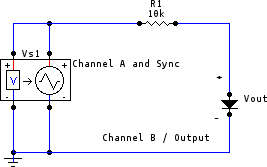
\includegraphics[width=\linewidth]{./1.png}
  \caption{Single Diode Clipping Circuit}
  \label{fig:circuit_1a}
  \end{center}
  \par\end{centering}
  \end{figure}

  \begin{figure}[htpb]
  \begin{centering}
  \begin{center}
  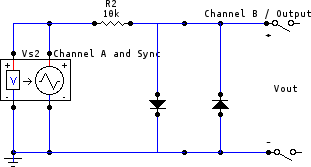
\includegraphics[width=\linewidth]{./2.png}
  \caption{Parallel Diode Clipping Circuit}
  \label{fig:circuit_1b}
  \end{center}
  \par\end{centering}
  \end{figure}

  \begin{figure}[htpb]
  \begin{centering}
  \begin{center}
  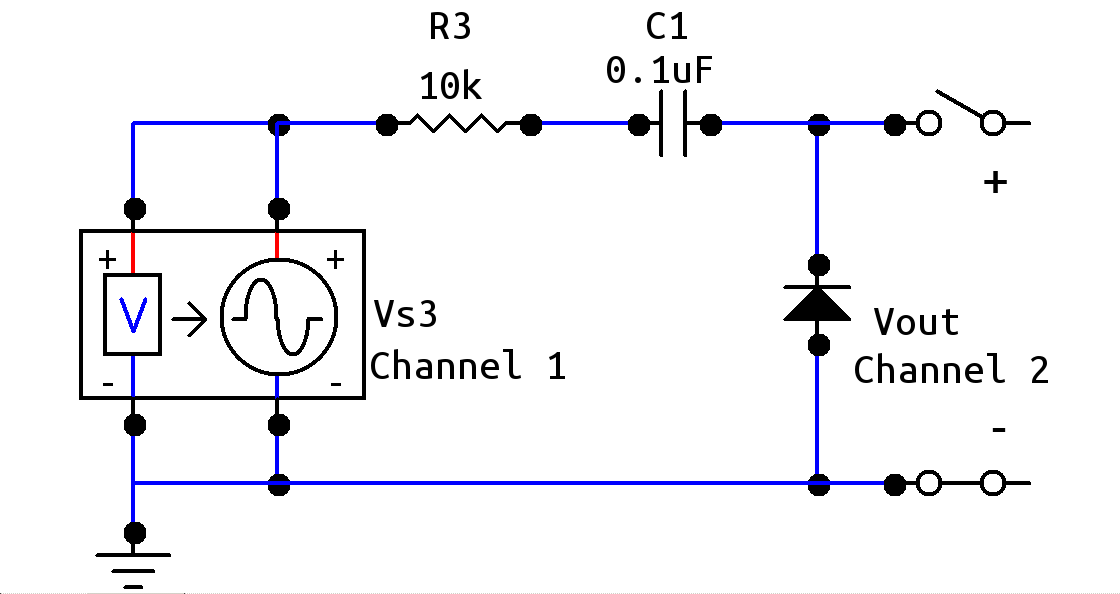
\includegraphics[width=\linewidth]{./3a.png}
  \caption{Clamping Circuit}
  \label{fig:circuit_2}
  \end{center}
  \par\end{centering}
  \end{figure}

  \begin{figure}[htpb]
  \begin{centering}
  \begin{center}
  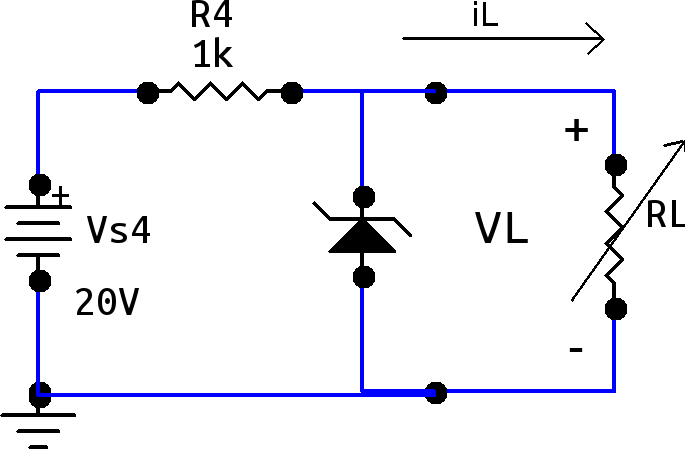
\includegraphics[width=\linewidth]{./3.png}
  \caption{Voltage Regulator Circuit}
  \label{fig:circuit_3}
  \end{center}
  \par\end{centering}
  \end{figure}

  \begin{figure}[htpb]
  \begin{centering}
  \begin{center}
  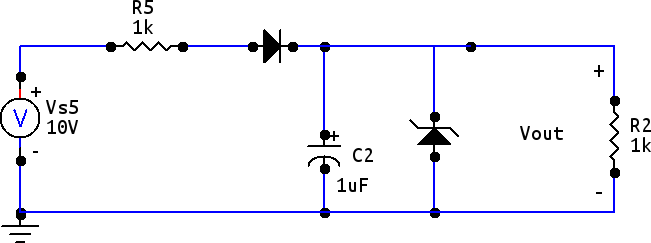
\includegraphics[width=\linewidth]{./acdc_circuit_diag.png}
  \caption{DC Power Supply Circuit Diagram}
  \label{fig:acdc_circuit_diag}
  \end{center}
  \par\end{centering}
  \end{figure}

  \begin{figure}[htpb]
  \begin{centering}
  \begin{center}
  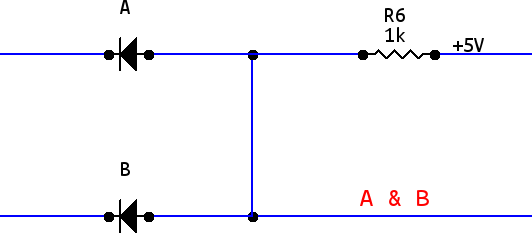
\includegraphics[width=\linewidth]{./and_gate.png}
  \caption{Logical AND Gate Circuit Diagram}
  \label{fig:and_gate_diagram}
  \end{center}
  \par\end{centering}
  \end{figure}

  \begin{figure}[htpb]
  \begin{centering}
  \begin{center}
  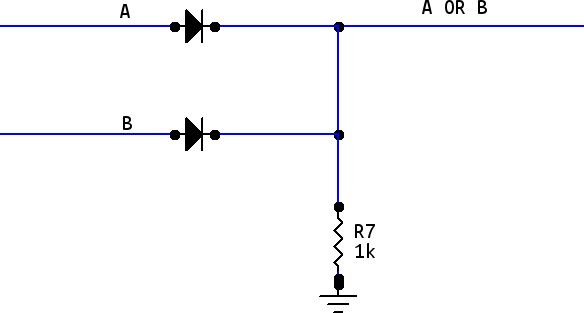
\includegraphics[width=\linewidth]{./or_gate.png}
  \caption{Logical OR Gate Circuit Diagram}
  \label{fig:or_gate_diagram}
  \end{center}
  \par\end{centering}
  \end{figure}

%\bibliographystyle{plain}
%\bibliography{physbib}

\end{document}